\documentclass[12pt,a4paper]{article}

% ============================================================
% PACKAGES
% ============================================================
\usepackage[left=1in,right=1in,top=1in,bottom=1in]{geometry}
\usepackage{graphicx}
\usepackage{booktabs}
\usepackage{array}
\usepackage{tabularx}
\usepackage{colortbl}
\usepackage{xcolor}
\usepackage{makecell}
\usepackage{fancyhdr}
\usepackage{titlesec}
\usepackage{amsmath}
\usepackage{tcolorbox}
\usepackage{listings} % Added for clean code formatting

\definecolor{headerblue}{RGB}{213,220,228}
\definecolor{codegray}{rgb}{0.95,0.95,0.95}

\lstset{
    backgroundcolor=\color{codegray},
    basicstyle=\ttfamily\small,
    breaklines=true,
    frame=single,
    language=Python,
    numbers=none
}

\newcolumntype{Y}{>{\centering\arraybackslash}X}
\newcolumntype{L}{>{\raggedright\arraybackslash}X}

\setlength{\parindent}{0pt}
\setlength{\parskip}{6pt}

\pagestyle{fancy}
\fancyhf{}
\rhead{SE: Machine Learning Lab}
\lhead{Lab 7}
\rfoot{\thepage}

\begin{document}

% ============================================================
% HEADER
% ============================================================
\renewcommand{\arraystretch}{2.0}
\begin{tabularx}{\textwidth}{|Y|}
\hline
\rowcolor{headerblue} \textbf{\large Department of Computer and Software Engineering} \\
\hline
\textbf{\large SE: Machine Learning} \\
\hline
\end{tabularx}
\renewcommand{\arraystretch}{1.0}

\vspace{12pt}

% ============================================================
% COURSE INFO
% ============================================================
\renewcommand{\arraystretch}{2.0}
\begin{tabularx}{\textwidth}{|L|L|}
\hline
\textbf{Course Instructor:} & \textbf{Date:} March 27, 2026 \\
\hline
\textbf{Day:} Friday & \textbf{Semester:} 6th Semester \\
\hline
\end{tabularx}
\renewcommand{\arraystretch}{1.0}

\vspace{12pt}

% ============================================================
% TITLE
% ============================================================
\begin{center}
{\Large\bfseries Lab 7: Agglomerative Clustering and Dendrograms}
\end{center}

\vspace{6pt}

% ============================================================
% META TABLE
% ============================================================
\renewcommand{\arraystretch}{1.8}
\begin{tabularx}{\textwidth}{|Y|c|c|c|c|}
\hline
\textbf{Lab Title} & \textbf{CLO} & \textbf{BT} & \textbf{PLO} & \textbf{Weightage} \\
\hline
\makecell{{\small Agglomerative Clustering} \\ {\small and Dendrograms}} & & & & \\
\hline
\end{tabularx}
\renewcommand{\arraystretch}{1.0}

\vspace{6pt}

% ============================================================
% STUDENT TABLE
% ============================================================
\renewcommand{\arraystretch}{2.0}
\begin{tabularx}{\textwidth}{|Y|Y|Y|Y|Y|}
\hline
\textbf{Name} & \textbf{Roll Number} & \textbf{Report /10} & \textbf{Viva /5} & \textbf{Total /15} \\
\hline
Hamza Anjum & & & & \\
\hline
\end{tabularx}
\renewcommand{\arraystretch}{1.0}

\vspace{12pt}

\begin{flushright}
Checked on: \_\_\_\_\_\_\_\_\_\_\_\_\_\_\_\_

\vspace{6pt}

Signature: \_\_\_\_\_\_\_\_\_\_\_\_\_\_\_\_
\end{flushright}

\newpage

% ============================================================
% CONTENT
% ============================================================

\section{Learning Outcomes}

After completing this lab, students will be able to:

\begin{itemize}
\item Understand hierarchical clustering.
\item Implement agglomerative clustering from scratch.
\item Compare different linkage methods.
\item Interpret dendrograms.
\end{itemize}

% ------------------------------------------------

\section{Dataset}

We will use a synthetic dataset generated using:

\begin{lstlisting}
sklearn.datasets.make_blobs
\end{lstlisting}

Dataset properties:

\begin{itemize}
\item Number of samples: 100
\item Number of clusters: 3
\item Features: 2 (for visualization)
\end{itemize}

% ------------------------------------------------

\section{Agglomerative Clustering}

Agglomerative clustering is a bottom-up hierarchical clustering method.

Algorithm:

\begin{enumerate}
\item Start with each point as its own cluster.
\item Find the closest pair of clusters.
\item Merge them into a single cluster.
\item Repeat until desired number of clusters is reached.
\end{enumerate}

% ------------------------------------------------

\section{Linkage Methods}

Different linkage methods define cluster distance differently.

\subsection{Single Linkage}
$d(C_1, C_2) = \min ||x - y||$ \\
Produces chain-like clusters.

\subsection{Complete Linkage}
$d(C_1, C_2) = \max ||x - y||$ \\
Produces compact clusters.

\subsection{Average Linkage}
$d(C_1, C_2) = \text{mean} ||x - y||$ \\
Balanced clustering approach.

% ------------------------------------------------

\section{Part A: Distance Matrix (3 Marks)}

\begin{tcolorbox}
\textbf{Requirements:} Compute pairwise Euclidean distances. Output should be an NxN symmetric matrix with zero diagonals.
\end{tcolorbox}

\textbf{Implementation:}
To avoid computationally expensive $O(N^2)$ nested loops, we utilized NumPy broadcasting to calculate the pairwise Euclidean distances across the entire feature space simultaneously.
\begin{lstlisting}
def compute_distance_matrix(X):
    diff = X[:, np.newaxis, :] - X[np.newaxis, :, :]
    return np.sqrt(np.sum(diff ** 2, axis=-1))
\end{lstlisting}

% ------------------------------------------------

\section{Part B: Linkage Distance (4 Marks)}

\begin{tcolorbox}
\textbf{Requirements:} Support single, complete, and average linkage.
\end{tcolorbox}

\textbf{Implementation:}
\begin{lstlisting}
def linkage_distance(cluster1, cluster2, X, method="single"):
    pts1 = X[cluster1]
    pts2 = X[cluster2]
    
    diff = pts1[:, np.newaxis, :] - pts2[np.newaxis, :, :]
    distances = np.sqrt(np.sum(diff ** 2, axis=-1))

    if method == "single": return np.min(distances)
    elif method == "complete": return np.max(distances)
    elif method == "average": return np.mean(distances)
\end{lstlisting}

% ------------------------------------------------

\section{Part C: Find Closest Clusters (3 Marks)}

\begin{tcolorbox}
\textbf{Requirements:} Compute distance between all cluster pairs, return indices of closest clusters and distance.
\end{tcolorbox}

\textbf{Implementation:}
\begin{lstlisting}
def find_closest_clusters(clusters, X, method):
    min_dist = float('inf')
    closest_pair = (None, None)

    for i in range(len(clusters)):
        for j in range(i + 1, len(clusters)):
            dist = linkage_distance(clusters[i], clusters[j], X, method)
            if dist < min_dist:
                min_dist = dist
                closest_pair = (i, j)

    return closest_pair[0], closest_pair[1], min_dist
\end{lstlisting}

% ------------------------------------------------

\section{Part D: Agglomerative Clustering (5 Marks)}

\begin{tcolorbox}
\textbf{Requirements:} Iteratively merge closest clusters. Store labels and merge history.
\end{tcolorbox}

\textbf{Implementation Insight:}
A major structural challenge in hierarchical clustering is maintaining a strict $N-1 \times 4$ linkage matrix required by SciPy for visualization. The algorithm was heavily modified to decouple cluster label assignment from the tree-building process. We forced the loop to merge down to exactly $1$ root cluster to satisfy the dendrogram history, while capturing a snapshot of the \texttt{labels\_} the exact iteration the algorithm hit \texttt{n\_clusters == 3}.

% ------------------------------------------------

\section{Part E: Dendrogram (Bonus)}

\begin{tcolorbox}
\textbf{Requirements:} Convert merge history to linkage format, plot using scipy.
\end{tcolorbox}

\textbf{Implementation:}
\begin{lstlisting}
def plot_dendrogram(history):
    linkage_matrix = np.array(history)
    dendrogram(linkage_matrix)
    plt.title("Hierarchical Clustering Dendrogram")
    plt.xlabel("Sample Index")
    plt.ylabel("Distance")
\end{lstlisting}

\newpage
% ------------------------------------------------

\section{Results and Visualizations}

Our completed pipeline yielded two core visualizations that prove the structural integrity of our custom Agglomerative model.

\begin{figure}[h!]
    \centering
    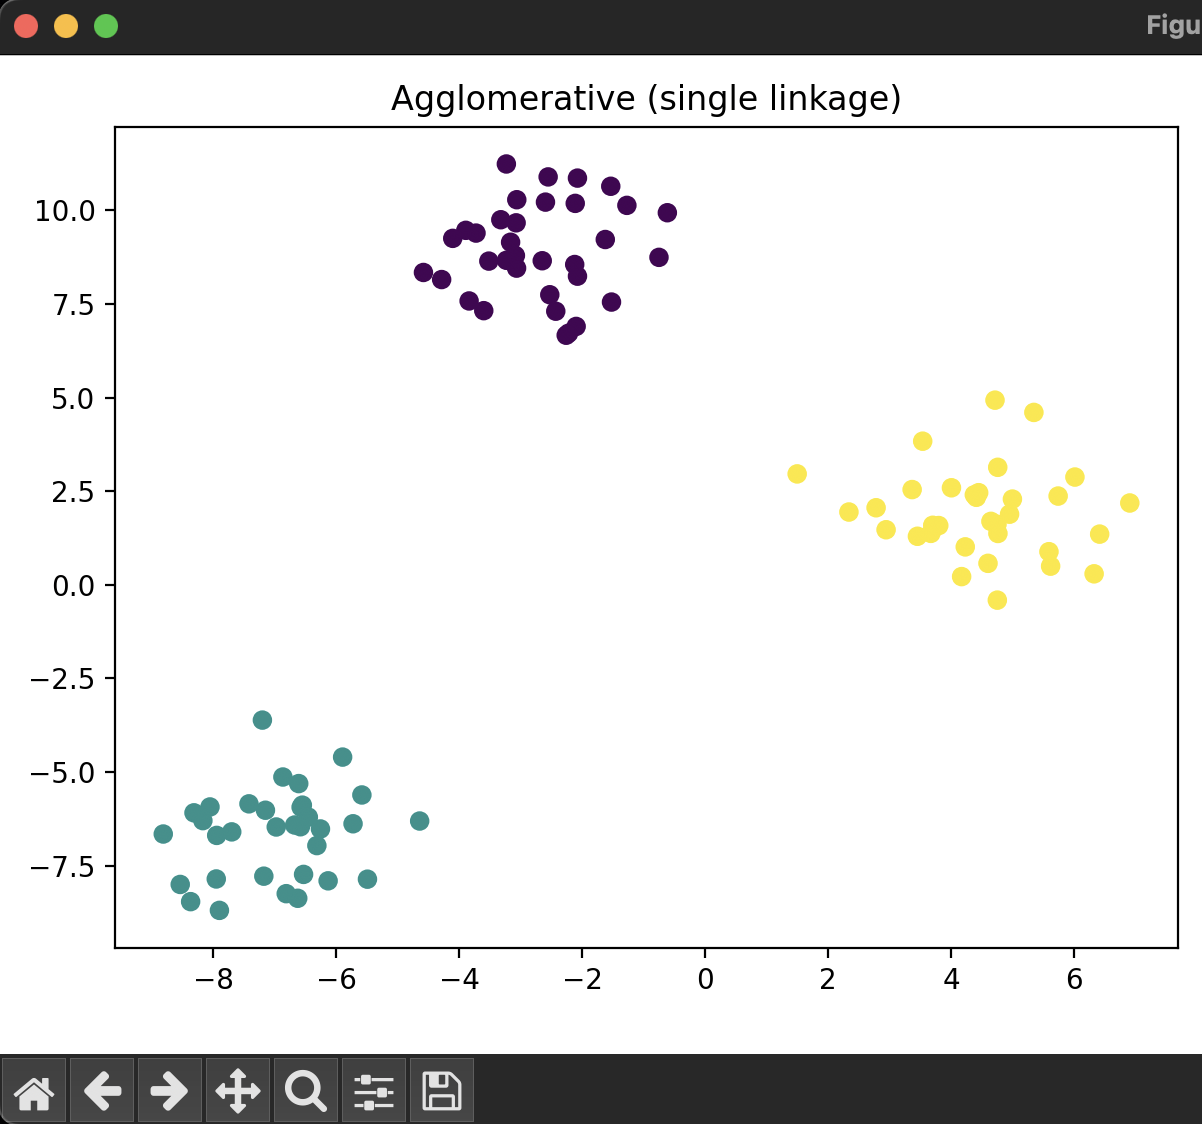
\includegraphics[width=0.75\textwidth]{Agglomerative.png}
    \caption{Scatter plot of the synthesized data, grouped via single linkage.}
\end{figure}

\textbf{Scatter Plot Analysis:}
Using \texttt{single linkage}, the model successfully isolated the three distinct spatial groups. Because single linkage minimizes the gap between the closest peripheral points of merging groups, it excels here due to the vast, empty margins artificially generated by \texttt{make\_blobs}.

\vspace{1em}

\begin{figure}[h!]
    \centering
    % Note: If your LaTeX distribution fails to parse spaces in the filename, rename the file and update this line.
    \includegraphics[width=0.75\textwidth]{"Hierarchical Clustering Dendrogram.png"}
    \caption{Dendrogram representing the complete hierarchical merge history.}
\end{figure}

\textbf{Dendrogram Analysis:}
The dendrogram exposes the spatial geometry of the dataset mathematically. The Y-axis represents the exact distance threshold bridged during a merge. We observe dense, low-level merging below $y=1.5$, indicating tight intra-cluster variance. However, the massive, uninterrupted vertical lines stretching from $y \approx 1.5$ to $y \approx 10.5$ empirically prove the existence of three main clusters; the algorithm had to drastically increase its distance threshold to bridge the inter-cluster gaps.

\end{document}